\documentclass{beamer}

%\usepackage[table]{xcolor}
\mode<presentation> {
  \usetheme{Boadilla}
%  \usetheme{Pittsburgh}
%\usefonttheme[2]{sans}
\renewcommand{\familydefault}{cmss}
%\usepackage{lmodern}
%\usepackage[T1]{fontenc}
%\usepackage{palatino}
%\usepackage{cmbright}
  \setbeamercovered{transparent}
\useinnertheme{rectangles}
}
%\usepackage{normalem}{ulem}
%\usepackage{colortbl, textcomp}
\setbeamercolor{normal text}{fg=black}
\setbeamercolor{structure}{fg= black}
\definecolor{trial}{cmyk}{1,0,0, 0}
\definecolor{trial2}{cmyk}{0.00,0,1, 0}
\definecolor{darkgreen}{rgb}{0,.4, 0.1}
\usepackage{array}
\newcommand{\argmin}{\arg\!\min}
\beamertemplatesolidbackgroundcolor{white}  \setbeamercolor{alerted
text}{fg=red}

\setbeamertemplate{caption}[numbered]\newcounter{mylastframe}

%\usepackage{color}
\usepackage{tikz}
\usetikzlibrary{arrows}
\usepackage{colortbl}
%\usepackage[usenames, dvipsnames]{color}
%\setbeamertemplate{caption}[numbered]\newcounter{mylastframe}c
%\newcolumntype{Y}{\columncolor[cmyk]{0, 0, 1, 0}\raggedright}
%\newcolumntype{C}{\columncolor[cmyk]{1, 0, 0, 0}\raggedright}
%\newcolumntype{G}{\columncolor[rgb]{0, 1, 0}\raggedright}
%\newcolumntype{R}{\columncolor[rgb]{1, 0, 0}\raggedright}

%\begin{beamerboxesrounded}[upper=uppercol,lower=lowercol,shadow=true]{Block}
%$A = B$.
%\end{beamerboxesrounded}}
\renewcommand{\familydefault}{cmss}
%\usepackage[all]{xy}

\usepackage{tikz}
\usepackage{lipsum}

 \newenvironment{changemargin}[3]{%
 \begin{list}{}{%
 \setlength{\topsep}{0pt}%
 \setlength{\leftmargin}{#1}%
 \setlength{\rightmargin}{#2}%
 \setlength{\topmargin}{#3}%
 \setlength{\listparindent}{\parindent}%
 \setlength{\itemindent}{\parindent}%
 \setlength{\parsep}{\parskip}%
 }%
\item[]}{\end{list}}
\usetikzlibrary{arrows}
%\usepackage{palatino}
%\usepackage{eulervm}
\usecolortheme{lily}
\newtheorem{com}{Comment}
\newtheorem{lem} {Lemma}
\newtheorem{prop}{Proposition}
\newtheorem{thm}{Theorem}
\newtheorem{defn}{Definition}
\newtheorem{cor}{Corollary}
\newtheorem{obs}{Observation}
 \numberwithin{equation}{section}

%\usepackage[latin1]{inputenc}
\title[Text as Data] % (optional, nur bei langen Titeln nötig)
{Text as Data}

\author{Justin Grimmer}
\institute[Stanford University]{Associate Professor\\Department of Political Science \\  Stanford University}
\vspace{0.3in}


\date{October 28th, 2014}%[Big Data Workshop] 
%\date{\today}


\begin{document}
\begin{frame}
\titlepage
\end{frame}


\begin{frame}
\frametitle{``Vanilla" Latent Dirichlet Allocation}

\begin{itemize}
\item[1)] Task: 
\begin{itemize}
\item[-] Discover thematic content of documents
\item[-] Quickly explore documents
\end{itemize}
\item[2)] Objective Function
\begin{eqnarray}
&& f(\boldsymbol{X}, \boldsymbol{\pi}, \boldsymbol{\Theta}, \boldsymbol{\alpha})  \nonumber 
\end{eqnarray}
Where:
\begin{itemize}
\item[-] $\boldsymbol{\pi} = N \times K$ matrix with row $\boldsymbol{\pi}_{i} = (\pi_{i1}, \pi_{i2}, \hdots, \pi_{iK}) \leadsto$ proportion of a document allocated to each topic
\item[-] $\boldsymbol{\Theta}$ = $K \times J$ matrix, with row $\boldsymbol{\theta}_{k} = (\theta_{1k}, \theta_{2k}, \hdots, \theta_{kJ})\leadsto$\alert{topics}
\item[-] $\boldsymbol{\alpha}$ = $K$ element long vector, population prior for $\boldsymbol{\pi}$.  
\end{itemize}
\item[3)] Optimization
\begin{itemize}
\item[-] Variational Approximation$\leadsto$ EM Algorithm where every step is an ``E" 
\item[-] Collapsed Gibbs Sampling$\leadsto$ MCMC algorithm
\item[-] \alert{Many} other variants  
\end{itemize}
\item[4)] Validation$\leadsto$ many of the same methods from clustering
\end{itemize}

\end{frame}







\begin{frame}
\frametitle{Topic and Mixed Membership Models}

\invisible<6->{\alert{Clustering}\\
 Document $\leadsto$ One Cluster}\\
\invisible<1-5>{\alert{Topic Models} (Mixed Membership) \\
Document $\leadsto$ Many clusters} 


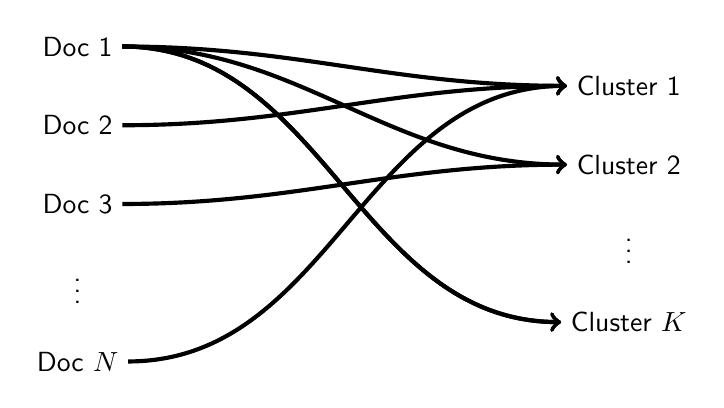
\begin{tikzpicture}

\node (doc1) at (-8,5.5) [] {Doc 1} ; 
\node (doc2) at (-8, 4.5) [] {Doc 2} ; 
\node (doc3) at (-8, 3.5) [] {Doc 3} ; 
\node (doc4) at (-8, 2.5) [] {$\vdots$} ; 
\node (doc5) at ( -8, 1.5) [] {Doc $N$} ; 


\node (clust1) at (-1, 5) [] {Cluster 1} ; 
\node (clust2) at (-1, 4) [] {Cluster 2} ; 
\node (clustd) at (-1, 3) [] {$\vdots$} ; 
\node (clust4) at (-1, 2) [] {Cluster $K$} ; 

\invisible<1,3->{\draw[->, line width = 1.5pt]  (doc1)  to [out=0, in=180] (clust4) ; } 
\invisible<1-2,4->{\draw[->, line width = 1.5pt]  (doc2)  to [out=0, in=180] (clust1) ; } 
\invisible<1-3,5->{\draw[->, line width = 1.5pt]  (doc3)  to [out=0, in=180] (clust2) ; } 
\invisible<1-4,6->{\draw[->, line width = 1.5pt]  (doc5)  to [out=0, in=180] (clust1) ; } 

\invisible<1-6>{\draw[->, line width= 1.5pt] (doc1) to [out=0, in =180] (clust1) ; 
\draw[->, line width= 1.5pt] (doc1) to [out=0, in =180] (clust2) ;
\draw[->, line width= 1.5pt] (doc1) to [out=0, in =180] (clust4) ;
}


\end{tikzpicture} 

\pause \pause \pause \pause \pause \pause 

\end{frame}


\begin{frame}
\frametitle{A Statistical Highlighter (With Many Colors) } 


\scalebox{0.45}{\includegraphics{WallachHighlighter.png}}

\end{frame}



\begin{frame}
\frametitle{Vanilla Latent Dirichlet Allocation$\leadsto$ Objective Function}

\begin{itemize}
\item[-] Consider document $i$, $(i =1, 2, \hdots, N)$.  
\invisible<1>{\item[-] Suppose there are $M_{i}$ total words and $\boldsymbol{x}_{i}$ is an $M_{i} \times 1$ vector, where $x_{im}$ describes the $m^{\text{th}}$ word used in the document$^{*}$.    }
\end{itemize}


\begin{eqnarray}
\invisible<1-6>{\boldsymbol{\theta}_{k} & \sim & \text{Dirichlet}(\boldsymbol{1}) \nonumber }\\
\invisible<1-7>{\alpha_{k} & \sim & \text{Gamma}(\alpha, \beta) \nonumber } \\
\invisible<1-3>{\boldsymbol{\pi}_{i}|\boldsymbol{\alpha} & \sim & \text{Dirichlet}(\boldsymbol{\alpha}) }\nonumber \\
\invisible<1-4>{\boldsymbol{\tau}_{im}| \boldsymbol{\pi}_{i} & \sim & \text{Multinomial}(1, \boldsymbol{\pi}_{i})} \nonumber \\
\invisible<1-5>{x_{im} | \boldsymbol{\theta}_{k}, \tau_{imk}=1 & \sim & \text{Multinomial}(1, \boldsymbol{\theta}_{k}) }\nonumber 
\end{eqnarray}


\invisible<1-2, 4->{$^{*}$Notice: this is a different representation than a document-term matrix.  $x_{im}$ is a number that says which of the $J$ words are used.  The difference is for clarity and we'll this representation is closely related to document-term matrix}


\pause \pause \pause \pause \pause \pause \pause 
\end{frame}


\begin{frame}
\frametitle{Vanilla Latent Dirichlet Allocation$\leadsto$ Objective Function}

Together the model implies the following posterior:

\begin{small}
\begin{eqnarray}
\invisible<1>{p(\boldsymbol{\pi}, \boldsymbol{T},\boldsymbol{\Theta}, \boldsymbol{\alpha}| \boldsymbol{X}) & \propto & \nonumber p(\boldsymbol{\alpha}) p(\boldsymbol{\pi}| \boldsymbol{\alpha}) p(\boldsymbol{T}| \boldsymbol{\pi}) p(\boldsymbol{X}| \boldsymbol{\theta}, \boldsymbol{T}) \nonumber } \\
\invisible<1-2>{& \propto & p(\boldsymbol{\alpha}) \prod_{i=1}^{N} \left[p(\boldsymbol{\pi}_{i} | \boldsymbol{\alpha}) \prod_{m=1}^{M_{i}} p(\boldsymbol{\tau}_{im}| \boldsymbol{\pi}) p(x_{im}| \boldsymbol{\theta}_{k}, \tau_{imk}=1) \right ] \nonumber }\\
\invisible<1-3>{& \propto & p(\boldsymbol{\alpha}) \prod_{i=1}^{N} \left[\alert<5>{\frac{\Gamma(\sum_{k=1}^{K} \alpha_{k})}{\prod_{k=1}^{K} \Gamma(\alpha_{k}) } \prod_{k=1}^{K} \pi_{ik}^{\alpha_{k}- 1}} \prod_{m=1}^{M}\prod_{k=1}^{K} \left[ \pi_{ik} \alert<6>{\prod_{j=1}^{J} \theta_{jk}^{x_{imj}} }  \right]^{\tau_{ikm}} \right] }\nonumber 
\end{eqnarray}

\end{small}

\invisible<1-6>{Optimization:} 
\begin{itemize}
\invisible<1-7>{\item[-] Variational Approximation$\leadsto$ Find ``closest" distribution} 
\invisible<1-8>{\item[-] Gibbs sampling $\leadsto$ MCMC algorithm to approximate posterior} 
\end{itemize}

\invisible<1-9>{\alert{Described in the slides appendix}} 
\pause \pause \pause \pause \pause \pause \pause \pause \pause 


\end{frame}


\begin{frame}
\frametitle{Running a Topic Model with Mallet}


{\tt to the Mallet/R Code!!}






\end{frame}


\begin{frame}
\frametitle{Why does this work$\leadsto$ Co-occurrence}


Where's the information for each word's topic? \pause \\

\invisible<1>{Reconsider document-term matrix} \pause 

\begin{center}
\invisible<1-2>{\begin{tabular}{ccccc}
\hline
        & $\text{Word}_1$ & $\text{Word}_2$ & $\hdots$ & $\text{Word}_J$ \\
\hline
Doc$_{1}$  & 0   & 1    & $\hdots$ & 0 \\
Doc$_{2}$ & 2 & 0  & $\hdots$ & 3\\
$\vdots$ & $\vdots$ & $\vdots$ & $\ddots$ & $\vdots$ \\
Doc$_{N}$ & 0 & 1 & $\hdots$ & 1 \\
\hline\hline
\end{tabular}} \pause 
\end{center}
\invisible<1-3>{Inner product of Documents (rows): $\textbf{Doc}_{i}^{'} \textbf{Doc}_{l} $} \pause \\
\vspace{0.1in}
\invisible<1-4>{Inner product of Terms (columns): $\textbf{Word}_j^{'} \textbf{Word}_k$ } \pause \\
\invisible<1-5>{\alert{Allows}: measure of correlation of term usage across documents (heuristically: partition words, based on usage in documents)} \pause \\
\invisible<1-6>{\alert{Latent Semantic Analysis}:  Reduce information in matrix using linear algebra (provides similar results, difficult to generalize)} \pause \\
\invisible<1-7>{\alert{Biclustering}: Models that partition documents and words simultaneously}   


\end{frame}


\begin{frame}
\frametitle{Why does this work$\leadsto$ Co-occurrence logic (h/t Colorado Reed Tutorial)}

\begin{eqnarray}
\only<1>{p(\boldsymbol{\pi}, \boldsymbol{T},\boldsymbol{\Theta}, \boldsymbol{\alpha}| \boldsymbol{X}) & \propto & \nonumber p(\boldsymbol{\alpha}) p(\boldsymbol{\pi}| \boldsymbol{\alpha}) p(\boldsymbol{T}| \boldsymbol{\pi}) p(\boldsymbol{X}| \boldsymbol{\theta}, \boldsymbol{T}) \nonumber  }
\only<2>{p(\boldsymbol{\pi}, \boldsymbol{T},\boldsymbol{\Theta}, \boldsymbol{\alpha}| \boldsymbol{X}) & \propto & \nonumber p(\boldsymbol{\alpha}) p(\boldsymbol{\pi}| \boldsymbol{\alpha}) p(\boldsymbol{T}| \boldsymbol{\pi}) \underbrace{p(\boldsymbol{X}| \boldsymbol{\theta}, \boldsymbol{T})}_{1} \nonumber  }
\only<3>{p(\boldsymbol{\pi}, \boldsymbol{T},\boldsymbol{\Theta}, \boldsymbol{\alpha}| \boldsymbol{X}) & \propto & \nonumber p(\boldsymbol{\alpha}) p(\boldsymbol{\pi}| \boldsymbol{\alpha}) \underbrace{p(\boldsymbol{T}| \boldsymbol{\pi})}_{2} \underbrace{p(\boldsymbol{X}| \boldsymbol{\theta}, \boldsymbol{T})}_{1} \nonumber  }
\only<4>{p(\boldsymbol{\pi}, \boldsymbol{T},\boldsymbol{\Theta}, \boldsymbol{\alpha}| \boldsymbol{X}) & \propto & \nonumber p(\boldsymbol{\alpha}) \underbrace{p(\boldsymbol{\pi}| \boldsymbol{\alpha})}_{3} \underbrace{p(\boldsymbol{T}| \boldsymbol{\pi})}_{2} \underbrace{p(\boldsymbol{X}| \boldsymbol{\theta}, \boldsymbol{T})}_{1} \nonumber  }
\end{eqnarray}

\begin{itemize}
\invisible<1>{\item[1)] $\boldsymbol{\theta} \leadsto$ Greater weight on terms that occur together} 
\invisible<1-2>{\item[2)] $\boldsymbol{\pi} \leadsto$ Greater weight on indicators that appear more regularly} 
\invisible<1-3>{\item[3)] $\boldsymbol{\alpha}\leadsto$ Emphasis on $\boldsymbol{\pi}$ with greater weight}
\end{itemize}

\pause \pause \pause 


\end{frame}







\begin{frame}
\frametitle{Validation$\leadsto$ Topic Intrusion}

Thursday$\leadsto$ discussed several validations

\begin{itemize}
\item[-] Labeling paragraphs
\begin{itemize}
\item[-] Identify separating words automatically
\item[-] Label topics manually (read!)
\end{itemize}
\item[-] Statistical methods
\begin{itemize}
\item[1)] Entropy
\item[2)] Exclusivity
\item[3)] Cohesiveness
\end{itemize}
\item[-] Experiment Based Methods
\begin{itemize}
\item[-] Word intrusion$\leadsto$ topic validity
\item[-] \alert{Topic intrusion}$\leadsto$ model fit
\end{itemize}

\end{itemize}



\end{frame}


\begin{frame}
\frametitle{Validation$\leadsto$ Topic Intrusion}


\begin{itemize}
\item[1)] Ask research assistant to read paragraph
\item[2)] Construct experiment
\begin{itemize}
\item[-] For the document, select top three topics
\item[-] Select a fourth topic
\item[-] Show participant, ask her/him to identify intruder
\end{itemize}

Higher identification$\leadsto$ topics are a better model of text


\end{itemize}

\end{frame}




\begin{frame}
\frametitle{Example 1: Japanese Campaign Manifestos (Catalinac 2011)} 


\begin{itemize}
\item[-] Why is Japan revising its constitution?
\item[-] \alert{IR} question: why is Japan now willing to engage militaristic foreign action?
\item[-] \alert{One explanation}: election reform in 1993, changed electoral incentives
\item[-] To answer well: characterize campaigns across 50 + years
\begin{itemize}
\item[-] \alert{That sounds hard} 
\item[-] \alert{That sounds impossible}
\end{itemize}
\item[-] Determined (relentless) data collection
\item[-] Latent Dirichlet Allocation (on japanese texts)
\end{itemize}


\end{frame}



\begin{frame}
\frametitle{Example 1: Japanese Campaign Manifestos (Catalinac 2011) } 


\only<1-3, 5->{
Japanese Elections: \pause 
\begin{itemize}
\invisible<1>{\item[-] Election Administration Commission runs elections $\rightarrow$ district level} \pause 
\invisible<1-2>{\item[-] Required to submit manifestos for all candidates to National Diet} \pause 
\invisible<1-4>{\item[-] Collected from 1950- 2009} \pause
\begin{itemize}
\invisible<1-5>{\item[-] Available only at district level} \pause
\invisible<1-6>{\item[-] \alert{Until}: 2009 national library made texts available on microfilm } \pause
\end{itemize}
\invisible<1-7>{\item[-] Collected from microfilm, hand transcribed (no OCR worked), used a variety of techniques to create a TDM } \pause
\invisible<1-8>{\item[-] \alert{Harder for Japanese} } 
\end{itemize}
}


\only<4>{
Typical Manifesto: 
\scalebox{0.45}{\includegraphics{Tokyo1.pdf}}}\pause 


\end{frame}

\begin{frame}
\frametitle{Example 1:  Japanese Campaign Manifestos (Catalinac 2014)}

\begin{itemize}
\item[-] Applies Vanilla LDA (using R Code I'll detail in a moment) 
\item[-] Output: topics (with Japanese characters)
\end{itemize}

\end{frame}


\begin{frame}
\frametitle{Example 1: Japanese Campaign Manifestos (Catalinac 2011)}

\scalebox{0.3}{\includegraphics{Topics.png} } 

\end{frame}


\begin{frame}
\frametitle{Example 1: Japanese Campaign Manifestos (Catalinac 2011)}

\only<1>{\scalebox{0.4}{\includegraphics{Pork.pdf} }}
\only<2>{\scalebox{0.4}{\includegraphics{NatSecurity.pdf}}}

\end{frame}


\begin{frame}

\scalebox{0.5}{\includegraphics{Cover1.jpg}}


\end{frame}




\begin{frame}
\frametitle{Example 2: Automated Literature Reviews} 

\alert{Recall}: literature reviews are hard to conduct\\
\alert{LDA}: developed (in part) to help structure {\tt JSTOR} database\\
Use {\tt JSTOR}'s research service to obtain data to analyze\\
\alert{Question:} How do scholars use classic text: \alert{Home Style}\\
Analysis: all articles that cite \alert{Home Style} in JSTOR's data\\

\end{frame}





\begin{frame}
\frametitle{Example 2: Automated Literature Reviews} 

Output: topic estimates
\begin{itemize}
\item[-] Obtain $\log \theta_k$ from model 
\item[-] One method to summarize a topic:
\begin{itemize}
\item[-] $\exp(\log \theta_k) $ (select 10-20 biggest words) 
\item[-] $\exp(\log \theta_k) - \text{Average}_{j\neq k} \exp(\log \theta_j)$ (select 10-20 biggest words) 
\end{itemize}
\end{itemize}


\end{frame}

\begin{frame}
\frametitle{Example 2: Automated Literature Reviews} 
Example topics:
\small
\begin{tabular}{lll} 
\hline\hline
Label & Stems & Proportion of Docs \\
\hline
Life Style & member,district,attent,congress,time,cohort,retir & 0.03  \\
Comp.Home & constitu,mp,member,parti,role,local,british &  0.02  \\
Casework & casework,district,constitu,variabl,staff,congression,fiorina & 0.03\\
Votes & vote,variabl,model,estim,measur,legisl,constitu & 0.04 \\
Id. Shirk & ideolog,vote,shirk,constitu,parti,senat,voter & 0.03\\
C. letters & mail,govern, activ,respond,commun,offic &  0.02\\
\hline 
\hline 
\end{tabular} 


\end{frame}

\begin{frame}
\frametitle{Example Document}


\only<1>{Wawro (2001) ``A Panel Probit Analysis of Campaign Contributions and Roll Call Votes"
\scalebox{0.4}{\includegraphics{Wawro.pdf}} } 
\only<2>{Bender (1996) ``Legislator Voting and Shirking  A Critical Review of the Literature" 
\scalebox{0.4}{\includegraphics{Bender.pdf}}}
\only<3>{Parker (1980) ``Cycles in Congressional District Attention" 
\scalebox{0.4}{\includegraphics{Parker.pdf}}}
\only<4>{Shepsle (1985) ``Policy Consequences of Government by Congressional Subcommittees" 
\scalebox{0.4}{\includegraphics{Shepsle.pdf}} }


\end{frame}




\begin{frame}
\frametitle{History of Home Style}



\begin{center}
\only<1>{\scalebox{0.4}{\includegraphics{Home1.pdf}} }
\only<2>{\scalebox{0.4}{\includegraphics{Home2.pdf}} } 
\only<3>{\scalebox{0.4}{\includegraphics{Home3.pdf}} }
\only<4>{\scalebox{0.4}{\includegraphics{Vote1.pdf}} }
\only<5>{\scalebox{0.4}{\includegraphics{Vote2.pdf}} } 
\only<6>{\scalebox{0.4}{\includegraphics{Vote3.pdf}} }
\end{center}


\end{frame}



\begin{frame}

\begin{center}
\scalebox{0.1}{\includegraphics{Cover2.jpg}}
\end{center}

\end{frame}


\begin{frame}

\begin{center}
What legislators claim (Grimmer, Westwood, Messing 2014) \pause \invisible<1>{$\leadsto$ LDA credit claiming press releases} 

\begin{footnotesize}
\begin{tabular}{lll}
\hline\hline
\invisible<1>{Labels & Key Words & Proportion}  \\
\hline
\invisible<1-2>{Requested appropriations&bill,funding,house,million,appropriations&0.08}   \\ 
\invisible<1-4>{Fire department grants&fire,grant,department,program,firefighters&0.08 } \\ 
\invisible<1-6>{Stimulus&recovery,funding,jobs,information, act, &0.06}   \\ 
\invisible<1-7>{Transportation&transportation,project,airport,transit,million&0.06}  \\ 
\end{tabular}
\end{footnotesize}
\end{center}


\invisible<1-2>{\only<1-3>{
``Dave Camp announced today that he was able to secure \$2.5 million for widening
M-72 from US-31 easterly 7.2 miles to Old M-72.  \alert{The
bill will now head to the Senate for consideration...We have two more hurdles to clear to make sure the money is in the bill when it
hits the President's desk: a vote in the Senate and a conference committee}" (Camp, 2005)}}


\only<4>{``Congressman Doc Hastings has boosted federal funding for work on the Columbia Basin water supply for next year. Hastings has added \$400,000 for work on the Odessa Subaquifer, which when combined with the funding in the President's budget request, totals \$1 million for Fiscal Year 2009"...``\alert{Hastings' funding for the Odessa Subaquifer and Potholes Reservoir was included in the Fiscal Year 2009 Energy and Water Appropriations bill which was approved today by the full House Appropriations Committee. (Hastings, 2008)}"}



\only<5>{``Maurice Hinchey (D-NY) today \alert{announced} that the West Endicott Fire Company has been awarded a \$17,051 federal grant to purchase approximately 10 sets of protective clothing, as well as radio equipment and air packs for its volunteer firefighters" (Hinchey, 2008) } 


\only<6>{``Congressman Pete Visclosky today \alert{announced} that the Crown Point Fire Department
will receive a \$16,550 Department of Homeland Security (DHS) grant to purchase a
modular portable video system" (Visclosky, 2008)}



\pause\pause \pause \pause \pause \pause 







\end{frame}





\begin{frame}
\frametitle{Correlated Topic Models}

Dirichlet distribution$\leadsto$ Assumes negative covariance between topics\\
\alert{Logistic Normal Distribution}$\leadsto$ Allows some positive covariance between topics\\

\begin{eqnarray}
\boldsymbol{\theta}_{k} & \sim & \text{Dirichlet}(\boldsymbol{1}) \nonumber \\
\boldsymbol{\eta}_{i}| \boldsymbol{\mu}, \boldsymbol{\Sigma} & \sim & \text{Multivariate Normal}(\boldsymbol{\mu}, \boldsymbol{\Sigma}) \nonumber \\
\boldsymbol{\pi}_{i}  & = & \frac{\exp\left(\boldsymbol{\eta}_{i}\right)}{\sum_{k=1}^{K} \exp\left(\eta_{ik}\right)} \nonumber \\
\boldsymbol{\tau}_{im} | \boldsymbol{\pi}_{i} & \sim & \text{Multinomial}(1, \boldsymbol{\pi}_{i}) \nonumber \\
x_{im} | \boldsymbol{\theta}_{k}, \tau_{imk} = 1 & \sim & \text{Multinomial}(1, \boldsymbol{\theta}_{k}) \nonumber 
\end{eqnarray}



\end{frame}



\begin{frame}
\frametitle{Vanilla Topic Models}

\begin{itemize}
\item[1)] Vanilla Topic Models
\item[2)] Structural Topic Models$\leadsto$ Different paths for validations
\end{itemize}



\end{frame}


\begin{frame}
\frametitle{Appendix: Estimating LDA}

\begin{itemize}
\item[1)] Variational Approximation
\item[2)] Collapsed Gibbs Sampling
\end{itemize}

\end{frame}


\begin{frame}
\frametitle{Variational Approximation}
Basic set up \pause \\
\invisible<1>{Call $q(\boldsymbol{\pi}, \boldsymbol{\theta},
\boldsymbol{T}, \boldsymbol{\alpha})$ an arbitrary distribution the \alert{approximating}
distribution.} \pause \invisible<1-2>{Recall $p(\boldsymbol{\pi},
\boldsymbol{\theta}, \boldsymbol{T}, \boldsymbol{\alpha}|
\boldsymbol{X})$ is the posterior} \pause \\
 \invisible<1-3>{Our goal is to make $q(\boldsymbol{\pi}, \boldsymbol{\theta},
\boldsymbol{T})$ as \alert{close} as possible to
$p(\boldsymbol{\pi}, \boldsymbol{\theta}, \boldsymbol{T},\boldsymbol{\alpha}|
\boldsymbol{X})$.}\pause
\begin{eqnarray}
\invisible<1-4>{q(\boldsymbol{\pi}, \boldsymbol{\theta},
\boldsymbol{T}, \boldsymbol{\alpha})^{*} & = & \text{arg min}_{q(\boldsymbol{\pi},
\boldsymbol{\theta}, \boldsymbol{T}, \boldsymbol{\alpha})} \text{KL}(q(\boldsymbol{\pi},
\boldsymbol{\theta}, \boldsymbol{T}, \boldsymbol{\alpha})) || p(\boldsymbol{\pi},
\boldsymbol{\theta}, \boldsymbol{T}, \boldsymbol{\alpha}| \boldsymbol{X})) ) \nonumber }
\pause
\end{eqnarray}
\invisible<1-5>{KL is the \alert{Kullback-Leibler} Divergence
between $q(\boldsymbol{\pi}, \boldsymbol{\theta}, \boldsymbol{T}, \boldsymbol{\alpha})$
and $p(\boldsymbol{\pi}, \boldsymbol{\theta}, \boldsymbol{T}, \boldsymbol{\alpha}|
\boldsymbol{X})$.} \pause
\begin{eqnarray}
\invisible<1-6>{ \text{KL}(q || p) & = & - \sum_{\boldsymbol{T}}
\iint q(\boldsymbol{T}, \boldsymbol{\pi}, \boldsymbol{\theta}, \boldsymbol{\alpha}) \log
\left \{ \frac{p(\boldsymbol{T}, \boldsymbol{\pi},
\boldsymbol{\theta}, \boldsymbol{\alpha} | \boldsymbol{X})}{q(\boldsymbol{T},
\boldsymbol{\pi}, \boldsymbol{\theta}, \boldsymbol{\alpha})} \right
\}d\boldsymbol{\pi}d\boldsymbol{\theta}} \nonumber
\end{eqnarray}
\pause
 \invisible<1-7>{KL-divergence measures \alert{dissimilarity}
between two distributions.}
\end{frame}



\begin{frame}
\frametitle{Variational Approximation}

Variational Approximation


\begin{eqnarray}
 q(\boldsymbol{\pi}, \boldsymbol{\theta},
\boldsymbol{T}, \boldsymbol{\alpha})^{*} & = & \text{arg min}_{q(\boldsymbol{\pi},
\boldsymbol{\theta}, \boldsymbol{T}, \boldsymbol{\alpha})} \text{KL}(q(\boldsymbol{\pi},
\boldsymbol{\theta}, \boldsymbol{T}, \boldsymbol{\alpha}) || p(\boldsymbol{\pi},
\boldsymbol{\theta}, \boldsymbol{T}, \boldsymbol{\alpha}| \boldsymbol{X}) ) \nonumber
\end{eqnarray} \pause
\invisible<1>{No assumptions about $q$} \pause \invisible<1-2>{then,
$q(\boldsymbol{\pi}, \boldsymbol{\theta}, \boldsymbol{T}, \boldsymbol{\alpha})^{*}
=p(\boldsymbol{\pi},
\boldsymbol{\theta}, \boldsymbol{T}, \boldsymbol{\alpha}| \boldsymbol{X})$ } \pause \\
\invisible<1-3>{\alert{Simplifying Assumption}: $q(\boldsymbol{\pi},
\boldsymbol{\theta}, \boldsymbol{T}, \boldsymbol{\alpha}) \equiv q(\boldsymbol{\pi})q(\boldsymbol{\theta})q(\boldsymbol{T})q(\boldsymbol{\alpha}).$} \pause \\
%\invisible<1-3>{Get more independence for free} \pause \\
%\invisible<1-4>{Why? \\
%$\boldsymbol{\pi} \perp \boldsymbol{\theta} | \boldsymbol{Y},
%\boldsymbol{T}$\\
%which is sufficient.  This implies, }\pause
% \invisible<1-5>{
%\begin{eqnarray}
%q(\boldsymbol{\pi}, \boldsymbol{\theta})q(\boldsymbol{T}) & =
%&q(\boldsymbol{\pi})q(\boldsymbol{\theta})q(\boldsymbol{T})
%\nonumber
%\end{eqnarray}}\pause
\invisible<1-4>{Sufficient to make inference tractable}\pause
\invisible<1-5>{\alert{!}}\pause \\
\invisible<1-6>{So, how do we minimize KL-divergence with respect to
$q(\boldsymbol{\pi})q(\boldsymbol{\theta})q(\boldsymbol{T})q(\boldsymbol{\alpha})$?}
\pause \\
\invisible<1-7>{We solve an equivalent maximization problem}
\end{frame}

\begin{frame}
\begin{eqnarray}
\log p(\boldsymbol{Y})  \pause \invisible<1>{& = & \log
\sum_{\boldsymbol{T}} \iint p(\boldsymbol{X}, \boldsymbol{T},
\boldsymbol{\pi}, \boldsymbol{\theta}, \boldsymbol{\alpha}) d\boldsymbol{\theta}
d\boldsymbol{\pi} } \nonumber \pause  \\
\invisible<1-2>{& = & \log \sum_{\boldsymbol{T}} \iint
\alert{\frac{q(\boldsymbol{\pi}, \boldsymbol{\theta},
\boldsymbol{T}, \boldsymbol{\alpha})}{q(\boldsymbol{\pi}, \boldsymbol{\theta},
\boldsymbol{T}, \boldsymbol{\alpha})}} p(\boldsymbol{X}, \boldsymbol{T},
\boldsymbol{\pi}, \boldsymbol{\theta}) d\boldsymbol{\theta}
d\boldsymbol{\pi} } \nonumber \pause \\
\invisible<1-3>{& \geq  & \sum_{\boldsymbol{T}} \iint
q(\boldsymbol{\pi}, \boldsymbol{\theta}, \boldsymbol{T}, \boldsymbol{\alpha}) \log
\left\{ \frac{p(\boldsymbol{X},\boldsymbol{T}, \boldsymbol{\pi},
\boldsymbol{\theta}, \boldsymbol{\alpha})}{q(\boldsymbol{\pi}, \boldsymbol{\theta},
\boldsymbol{T}, \boldsymbol{\alpha})}\right\}d\boldsymbol{\pi} d\boldsymbol{\theta}}
\nonumber \pause
\end{eqnarray}
\invisible<1-4>{$\sum_{\boldsymbol{T}} \iint q(\boldsymbol{\pi},
\boldsymbol{\theta}, \boldsymbol{T}, \boldsymbol{\alpha}) \log \left\{
\frac{p(\boldsymbol{X},\boldsymbol{T}, \boldsymbol{\pi},
\boldsymbol{\theta}, \boldsymbol{\alpha})}{q(\boldsymbol{\pi}, \boldsymbol{\theta},
\boldsymbol{T}, \boldsymbol{\alpha})}\right\}d\boldsymbol{\pi} d\boldsymbol{\theta}  =
\mathcal{L}(q) $}
\end{frame}

\begin{frame}
\begin{eqnarray}
\log p(\boldsymbol{Y}) & = &  \pause \invisible<1>{ \text{KL}(q||p)
+ \mathcal{L}(q) } \nonumber
\end{eqnarray}
\end{frame}

\begin{frame}
\begin{eqnarray}
\underbrace{\log p(\boldsymbol{Y})}_{\text{Fixed Number} }& = &
\text{KL}(q||p) + \mathcal{L}(q) \nonumber
\end{eqnarray}
\pause \invisible<1>{If $\mathcal{L}(q)$ increases} \pause
\invisible<1-2>{ then KL$(q||p)$ \alert{must} decrease.} \pause \\
\invisible<1-3>{Choose $q$ to maximize $\mathcal{L}(q)$} \pause
\invisible<1-4>{equivalent to minimizing KL$(q||p)$}.
\end{frame}

\begin{frame}
Iterative algorithm to maximize $\mathcal{L}(q)$. \pause \\
\invisible<1>{Initialize $q(\boldsymbol{\pi})^{\text{old}}$,
$q(\boldsymbol{\theta})^{\text{old}}$,
$q(\boldsymbol{T})^{\text{old}}$, and $q(\boldsymbol{\alpha}^{\text{old}}$) } \pause \\
\invisible<1-2>{Find \alert{$q(\boldsymbol{\pi})^{\text{new}}$} to
max $\mathcal{L}(q)$-- holding
$q(\boldsymbol{\theta})^{\text{old}}$, and
$q(\boldsymbol{T})^{\text{old}}$ \alert{constant}}\pause \\
\invisible<1-3>{Find $q(\boldsymbol{\theta})^{\text{new}}$ to max
$\mathcal{L}(q)$-- holding $q(\boldsymbol{T})^{\text{old}}$, and
$q(\boldsymbol{\pi})^{\text{new}}$ constant}\pause \\
\invisible<1-4>{Find $q(\boldsymbol{T})^{\text{new}}$ to max
$\mathcal{L}(q)$-- holding $q(\boldsymbol{\theta})^{\text{new}}$,
and $q(\boldsymbol{\pi})^{\text{new}}$ constant} \pause \\
\invisible<1-5>{Assume $q(\boldsymbol{\alpha})$ is degenerate, maximization step} \pause \\
\invisible<1-6>{Guaranteed convergence: $\mathcal{L}(q)$ is convex
in $q(\boldsymbol{\pi})$, $q(\boldsymbol{\theta})$,and
$q(\boldsymbol{T})$}
\end{frame}

\begin{frame}
Finding $q(\boldsymbol{\pi})^{\text{new}}$. \pause  \\

\invisible<1>{
\begin{eqnarray}
\mathcal{L}(q) & = & \int q(\boldsymbol{\pi})^{\text{new}}
\textcolor{blue}{\underbrace{\left\{\sum_{\boldsymbol{T}} \int \log
p(\boldsymbol{X}, \boldsymbol{T}, \boldsymbol{\theta},
\boldsymbol{\pi})q(\boldsymbol{T}, \boldsymbol{\alpha})^{\text{old}}
q(\boldsymbol{\theta})^{\text{old}} d\boldsymbol{\theta} \right
\}}_{\text{E}_{\boldsymbol{T}, \boldsymbol{\theta}}[\log
p(\boldsymbol{Y}, \boldsymbol{T}, \boldsymbol{\pi},
\boldsymbol{\theta})] }}d\boldsymbol{\pi} \nonumber
\\
& -&   \int q(\boldsymbol{\pi})^{\text{new}} \log
q(\boldsymbol{\pi})^{\text{new}} d\boldsymbol{\pi} +
\alert{\text{constants}}\nonumber
\end{eqnarray}
} \pause
\begin{eqnarray}
\invisible<1-2>{
 \textcolor{blue}{\log \tilde p (\boldsymbol{\pi})} =
 \textcolor{blue}{
\text{E}_{\boldsymbol{T}, \boldsymbol{\theta}}[\log
p(\boldsymbol{X}, \boldsymbol{T}, \boldsymbol{\pi},
\boldsymbol{\theta}, \boldsymbol{\alpha})]} + \textcolor{red}{\text{constants}} }
\nonumber
\end{eqnarray}



\end{frame}

\begin{frame}
Substituting in $ \textcolor{blue}{\log \tilde p
(\boldsymbol{\pi})}$,
\begin{eqnarray}
& = & \int q(\boldsymbol{\pi})^{\text{new} } \log \left(\frac{
\textcolor{blue}{\tilde p(\boldsymbol{\pi})}
}{q(\boldsymbol{\pi})^{\text{new}} } \right)d\boldsymbol{\pi}
\nonumber \pause  \\
\invisible<1>{& = & -
\text{KL}(q(\boldsymbol{\pi})^{\text{new}}||\textcolor{blue}{\tilde
p(\boldsymbol{\pi})}) \nonumber }
\end{eqnarray}
\pause \invisible<1-2>{At a maximum when
$q(\boldsymbol{\pi})^{\text{new}} = \textcolor{blue}{\tilde
p(\boldsymbol{\pi})}$ }\pause \\
\invisible<1-3>{Equivalently,
\begin{eqnarray}
\log q(\boldsymbol{\pi})^{\text{new}}
& = &  \log  \textcolor{blue}{\tilde p(\boldsymbol{\pi})} \nonumber \\
& = &  \textcolor{blue}{\text{E}_{\boldsymbol{T}, \boldsymbol{\theta}}[\log
p(\boldsymbol{X}, \boldsymbol{T}, \boldsymbol{\pi},
\boldsymbol{\theta}, \boldsymbol{\alpha})]}  + \textcolor{red}{\text{constants}} \nonumber
\end{eqnarray}}
\pause \invisible<1-4>{Or,} \pause
\invisible<1-5>{
\begin{eqnarray}
q(\boldsymbol{\pi})^{\text{new}} & = & \frac{\exp\left\{\textcolor{blue}{\text{E}_{\boldsymbol{T}, \boldsymbol{\theta}}[\log
p(\boldsymbol{X}, \boldsymbol{T}, \boldsymbol{\pi},
\boldsymbol{\theta}, \boldsymbol{\alpha})]} \right\}}{\int \exp\left\{\textcolor{blue}{\text{E}_{\boldsymbol{T}, \boldsymbol{\theta}}[\log
p(\boldsymbol{X}, \boldsymbol{T}, \boldsymbol{\pi},
\boldsymbol{\theta}, \boldsymbol{\alpha})]} \right\} d\boldsymbol{\pi}  } \nonumber
\end{eqnarray}
}

\end{frame}


\begin{frame}
Algorithm\ \\
  \pause \invisible<1>{Initialize
$q(\boldsymbol{\pi})^{\text{old}}$,
$q(\boldsymbol{\theta})^{\text{old}}$, and
$q(\boldsymbol{T})^{\text{old}}$ } \pause
\begin{eqnarray}
\invisible<1-2>{\log q(\boldsymbol{\pi})^{\text{new}} &  = &
\text{E}_{\boldsymbol{T}, \boldsymbol{\theta}}[ \log
p(\boldsymbol{X}, \boldsymbol{T}, \boldsymbol{\theta}, \boldsymbol{\pi}, \boldsymbol{\alpha}) ] + \text{constants} \nonumber} \pause \\
\invisible<1-3>{\log q(\boldsymbol{\theta})^{\text{new}} & = &
\text{E}_{\boldsymbol{T}, \boldsymbol{\pi}}[ \log p(\boldsymbol{X},
\boldsymbol{T}, \boldsymbol{\theta}, \boldsymbol{\pi}, \boldsymbol{\alpha}) ] +
\text{constants} \nonumber} \pause \\
\invisible<1-4>{\log q(\boldsymbol{T})^{\text{new}} & = &
\text{E}_{\boldsymbol{\theta}, \boldsymbol{\pi} }[ \log
p(\boldsymbol{Y}, \boldsymbol{T}, \boldsymbol{\theta},
\boldsymbol{\pi}, \boldsymbol{\alpha}) ] + \text{constants} \nonumber}
\end{eqnarray}

\pause \invisible<1-5>{All expectations over \alert{approximating}
distribution.} \pause \\

 \invisible<1-6>{To compute, rely on factorization in posterior}
\end{frame}

\begin{frame}
\frametitle{Variational Approximation Update Steps}

Carrying out the expectations, we obtain the following forms$\leadsto$ derivation \alert{not} assumption

\begin{eqnarray}
q(\boldsymbol{\tau}_{im}) & = & \text{Multinomial}(1, \boldsymbol{r}_{im}) \nonumber \\
q(\boldsymbol{\theta}_{k} ) &  = & \text{Dirichlet}(\boldsymbol{\eta}_{k}) \nonumber \\
q(\boldsymbol{\pi}_{i}) & = & \text{Dirichlet}(\boldsymbol{\gamma}_{i}) \nonumber 
\end{eqnarray}


\end{frame}

\begin{frame}
\frametitle{Update for $q(\boldsymbol{\tau}_{im})$}

Consider document $i$, word $m$, topic $k$
\begin{eqnarray}
r_{imk} & \propto & \exp\left(I(x_{im} = j) E[\log  \eta_{kj} ] + E[\log \gamma_{ik}] \right)\nonumber \\
& \propto & \exp\left(I(x_{im} = j) \left[\Psi(\eta_{kj}) - \Psi(\sum_{l=1}^{J} \eta_{kl})\right]  + \Psi(\gamma_{ik}) - \Psi(\sum_{m=1}^{K} \gamma_{im})) \right) \nonumber 
\end{eqnarray}

where $\Psi(\cdot)$ is the digamma function (the derivative of the gamma function)


\end{frame}

\begin{frame}
\frametitle{Update for $q(\boldsymbol{\eta}_{k})$}

Consider word $j$ and topic $k$, then, 
\begin{eqnarray}
\eta_{jk} & \propto & 1 + \sum_{i=1}^{N} \sum_{m=1}^{M_{i}} r_{imk} x_{im} \nonumber 
\end{eqnarray}


\end{frame}


\begin{frame}
\frametitle{Update for $q(\boldsymbol{\gamma}_{i})$}

Consider word topic $k$ and document $i$ 

\begin{eqnarray}
\gamma_{ik} & \propto & \alpha_{k} +  \sum_{m=1}^{M_{i}} r_{imk} \nonumber 
\end{eqnarray}


\end{frame}

\begin{frame}
\frametitle{Update for $\boldsymbol{\alpha})$}

Fast Newton-Raphson Algorithm
\end{frame}

\end{document}